\section{Ceph Filesystem}

%\subsection{System Architecture}

\begin{frame}{System Architecture}
    \begin{figure}[htpb]
        \centering
        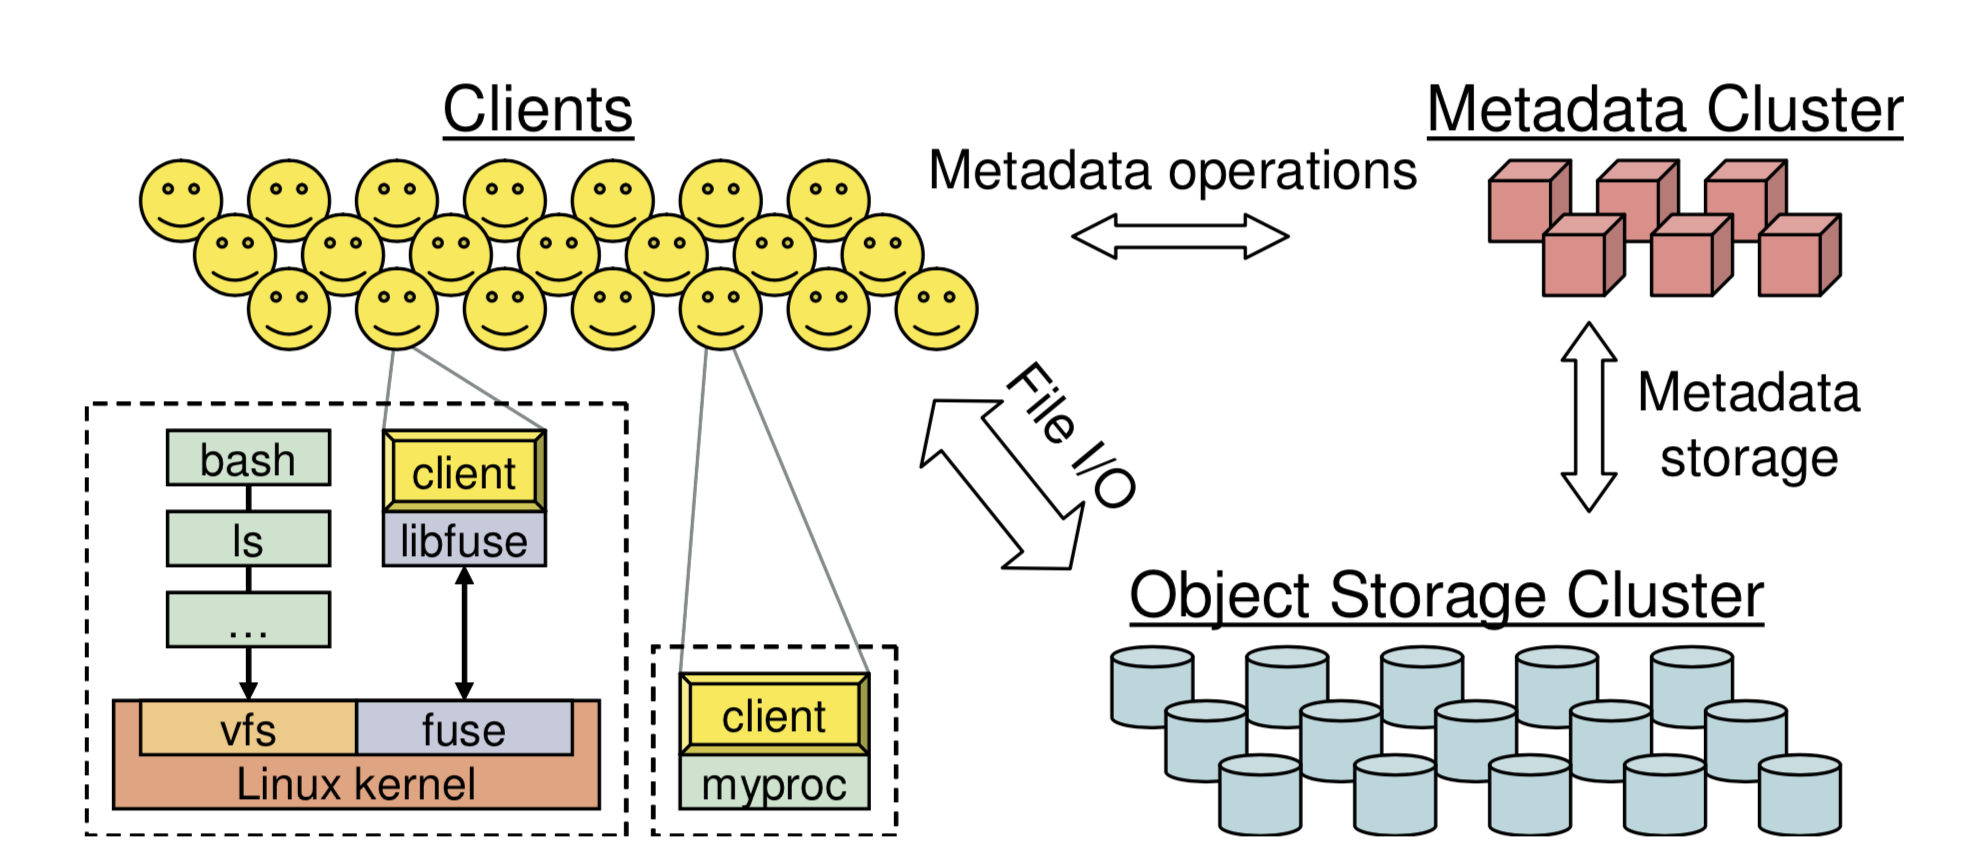
\includegraphics[width=0.8\linewidth]{cephfs-architecture.png}
    \end{figure}
\end{frame}

\begin{frame}{System Architecture}
    \begin{itemize}
        \item \textbf{Clients}
            \begin{itemize}
                \item Export a near-POSIX file system interface
            \end{itemize}
        \item \textbf{Cluster of OSDs}
            \begin{itemize}
                \item Store all data and metadata
                \item Communicate directly with clients
            \end{itemize}
        \item \textbf{Metadata Server Cluster}
            \begin{itemize}
                \item Manages the namespace (files + directories)
                \item Security, consistency and coherence
            \end{itemize}
    \end{itemize}
\end{frame}

\begin{frame}{Key Ideas}
    \begin{itemize}
        \item \textbf{Seperate data and metadata management tasks}
        \item \textbf{Dynamic partitioning of metadata data tasks inside metadata cluster}
            \begin{itemize}
                \item Avoid hot spots
            \end{itemize}
        \item \textbf{Let OSDs handle file migration and replication tasks}
    \end{itemize}
\end{frame}

%\subsection{Ceph Metadata Server}

\begin{frame}[fragile]{Create and Mount CephFS}
\begin{lstlisting}[language=python]
## creating pools
$ ceph osd pool create cephfs_data 128
$ ceph osd pool create cephfs_metadata 128
## creating a file system
$ ceph fs new cephfs cephfs_metadata cephfs_data
$ ceph fs ls
name: cephfs, metadata pool: cephfs_metadata, data pools: [cephfs_data ]
\end{lstlisting}

\begin{lstlisting}[language=python]
## there are 2 ways to mount a file system
## ceph-fuse is most of the time slower than the cephfs kernel module

## mount cephfs with the kernel driver
$ sudo mkdir /mnt/mycephfs
$ sudo mount -t ceph 192.168.0.1:6789:/ /mnt/mycephfs

## mount cephfs using fuse
$ sudo mkdir /home/username/cephfs
$ sudo ceph-fuse -m 192.168.0.1:6789 /home/username/cephfs
\end{lstlisting}
\end{frame}

\begin{frame}{MDS High Availabilty}
    \begin{itemize}
        \item MDSs can be running in two modes
            \begin{itemize}
                \item active
                \item standby
            \end{itemize}
        \item A standby MDS can become active
            \begin{itemize}
                \item If the previously active daemon goes away
            \end{itemize}
        \item Multiple active MDSs for load balancing
            \begin{itemize}
                \item Are a possibility
                \item This configuration is currently not supported/recommended
            \end{itemize}
    \end{itemize}
\end{frame}

\begin{frame}{MDS Functionality}
    \begin{itemize}
        \item The client learns about MDSs and OSDs from MON
            \begin{itemize}
                \item via MON Map, OSD Map and MDS Map
            \end{itemize}
        \item Clients talk to MDS for access to Metadata
            \begin{itemize}
                \item Permission bits, ACLs, file ownership, etc.
            \end{itemize}
        \item Clients talk to OSD for access to data
        \item MDSs themselves store all their data in OSDs
            \begin{itemize}
                \item In a separate pool called metadata
            \end{itemize}
    \end{itemize}
\end{frame}

\begin{frame}{MDS Functionality}
    \begin{figure}[htpb]
        \centering
        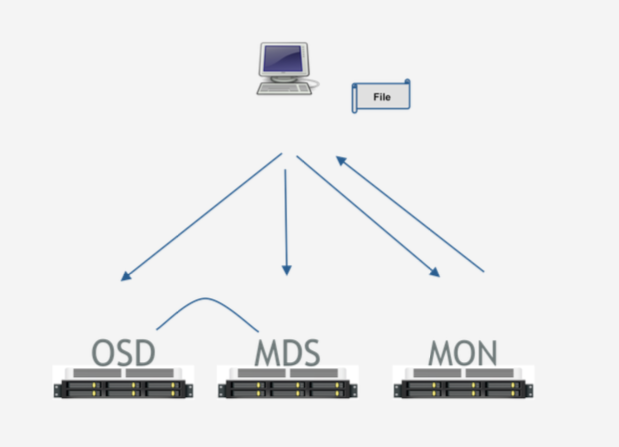
\includegraphics[width=0.8\linewidth]{cephfs-mds.png}
    \end{figure}
\end{frame}

\begin{frame}{Client Access Example}
    \begin{itemize}
        \item Client sends open request to MDS
        \item MDS returns capability, file inode, file size and stripe information
            \begin{itemize}
                \item capability specifies authorized operations on file
            \end{itemize}
        \item Client read/write directly from/to OSDs
        \item MDS manages the capability
        \item Client sends close request, relinquishes capability, provides details to MDS
    \end{itemize}
\end{frame}

%\subsection{Dynamic Tree Partitioning}

\begin{frame}{Metadata management}
    \begin{itemize}
        \item Metadata operations often make up as much as half of file system workloads...
        \item \textbf{Dynamic Subtree Partitioning}
            \begin{itemize}
                \item Lets Ceph dynamically share metadata workload among tens or hundreds of metadata servers(MDSs)
                \item Sharing is dynamic and based on current access patterns
            \end{itemize}
        \item Results in near-linear performance scaling in the number of MDSs
    \end{itemize}
\end{frame}

%\begin{frame}{Storing metadata}
%    \begin{itemize}
%        \item Most requests likely to be satisfied from MDS in-memory cache
%        \item Each MDS lodges its update operations in lazily-flushed journal
%            \begin{itemize}
%                \item Facilitates recovery
%            \end{itemize}
%        \item Directories
%            \begin{itemize}
%                \item Include i-nodes
%                \item Stored on a OSD cluster
%            \end{itemize}
%    \end{itemize}
%\end{frame}
%
%\begin{frame}{Dynamic Subtree Partitioning}
%    \begin{itemize}
%        \item Ceph uses primary copy approach to cached metadata management
%        \item Ceph adaptively distributes cached metadata across MDS nodes
%            \begin{itemize}
%                \item Each MDS measures popularity of data within a directory
%                \item Ceph migrates and/or replicates hot spots
%            \end{itemize}
%    \end{itemize}
%\end{frame}

\begin{frame}{Mapping Subdirectories to MDSs}
    \begin{figure}[htpb]
        \centering
        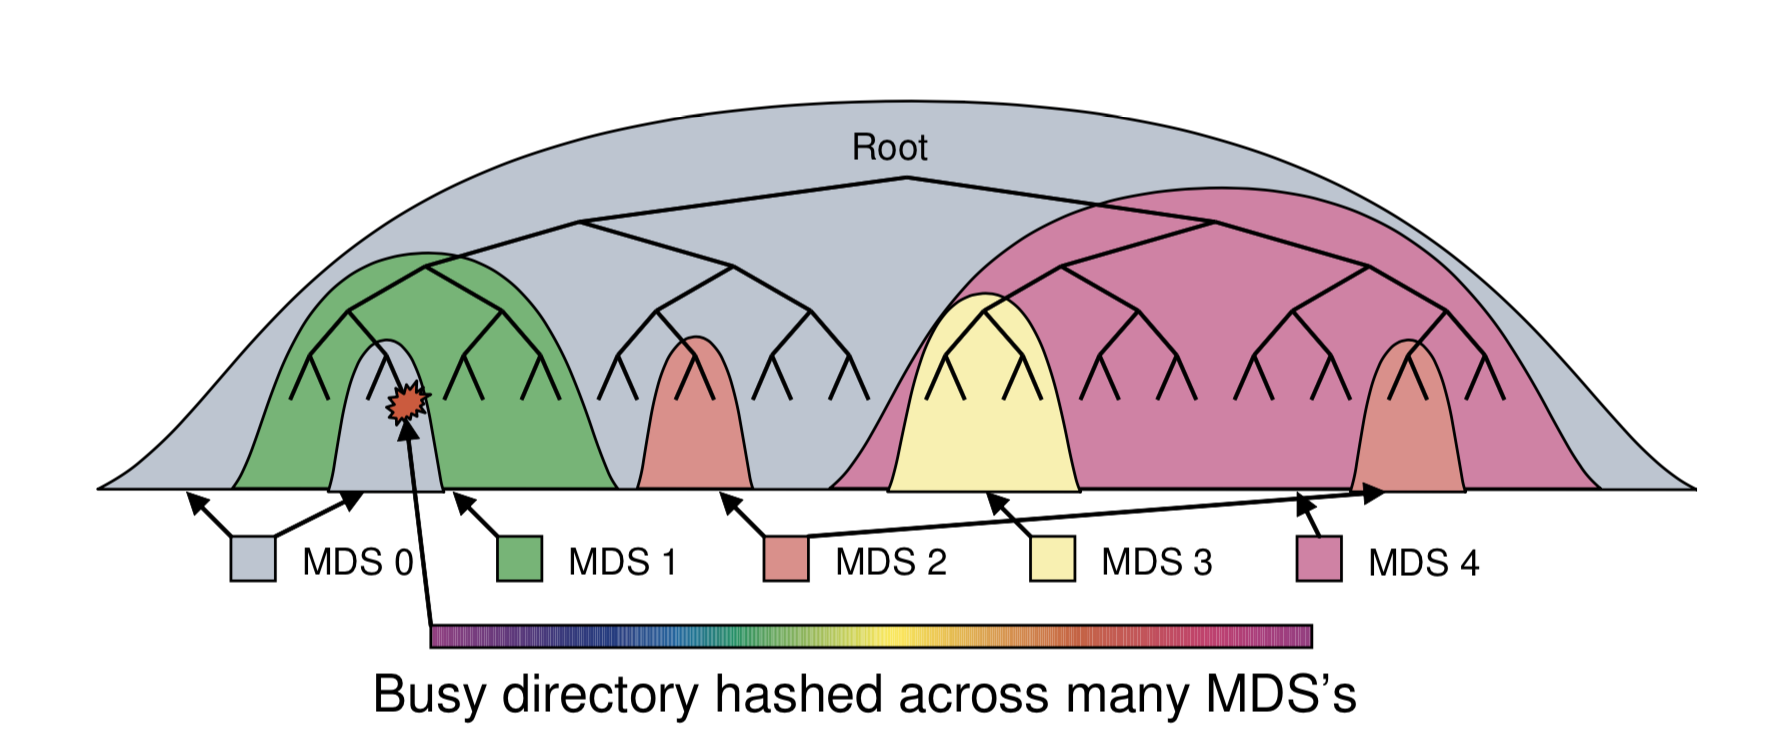
\includegraphics[width=0.8\linewidth]{cephfs-dtp.png}
    \end{figure}
\end{frame}

\begin{frame}[fragile]
\begin{columns}
    \begin{column}{0.4\textwidth}
\begin{lstlisting}[language=python]
apiVersion: v1
kind: PersistentVolume
metadata:
  name: cephfs-pv
spec:
  capacity:
    storage: 10Gi
  accessModes:
    - ReadWriteMany
  cephfs:
    monitors:
    - '172.31.56.105:6789'
    - '172.31.57.232:6789'
    - '172.31.58.195:6789'
    user: admin
    secretRef:
      name: ceph-secret
    readOnly: false
\end{lstlisting}

\begin{lstlisting}[language=python]
kind: PersistentVolumeClaim
apiVersion: v1
metadata:
  name: cephfs-pv-claim
spec:
  accessModes:
    - ReadWriteMany
  resources:
    requests:
      storage: 10Gi
\end{lstlisting}
    \end{column}
    \begin{column}{0.4\textwidth}
      
\begin{lstlisting}[language=python]
apiVersion: v1
kind: Pod
metadata:
  labels:
    test: cephfs-pvc-pod
  name: cephfs-pv-pod1
spec:
  containers:
  - name: cephfs-pv-busybox1
    image: busybox
    command: ["sleep", "60000"]
    volumeMounts:
    - mountPath: "/mnt/cephfs"
      name: cephfs-vol1
      readOnly: false
  volumes:
  - name: cephfs-vol1
    persistentVolumeClaim:
      claimName: cephfs-pv-claim
\end{lstlisting}
    \end{column}
\end{columns}
\end{frame}

